\subsection{Early work on unsupervised morphology induction}
Unsupervised approaches for morphology induction have been developed for a long time. In fact, competitions around this subject have been organized for several years\footnote{The "Morpho Challenge": \url{http://research.ics.aalto.fi/events/morphochallenge/}} and have resulted in evaluation resources for a few languages as well as empirical surveys of the performance of early algorithms. Most early approaches rely on the minimum description length (MDL) principle introduced by \cite{goldsmith2001}, which can be described as follows: the amount of information contained in the vocabulary of a given language is not proportional to its size, but rather to the size of the vocabulary of base forms (stems) plus the size of the grammar which describes how each form can be inflected. Therefore, MDL approaches seek to minimize approximate measures of the amount of information contained in these two parts. In practice, this is often done by defining an objective and using heuristic search techniques to minimize its value. This method, although relatively efficient, is unsatisfying because of its lack of flexibility: it is difficult to integrate more information in the model, be it linguistic knowledge, small amounts of labelled training data or context dependencies. Furthermore, these MDL models are in general trained on vocabularies and not corpora; word frequency is completely ignored because it is hard to integrate in this framework.

\subsection{Bayesian models for morphology induction}
Recently, more flexible approaches based on Bayesian inference have been proposed and shown to be capable of incorporating context information, agreement constraints \cite{lee2011, sirts2012} and prior linguistic knowledge \cite{chahuneau13}. In particular, \cite{goldwater2011} explain how to integrate both words as observed in a vocabulary (types) and in a corpus (tokens) in these models. They do so by considering a simple generative model of morphology which assumes that each word has a prefix and a (possibly empty) suffix, which we use as our base model for this project. Although this model is not able to capture general morphological phenomena in all possible languages, its structure is general enough that our discussion in this report is revelant to more advanced variations of this model\footnote{We justify this in more details in the future work section}.

\begin{figure}[h]
  \centering
  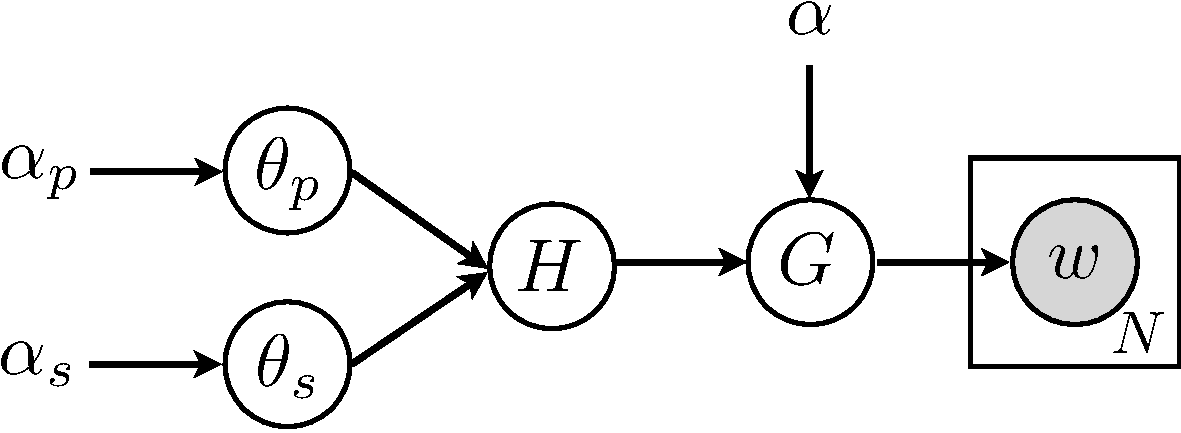
\includegraphics[width=0.6\textwidth]{fig/v1}
  \caption{Baseline model proposed by \cite{goldwater2011}}
  \label{fig:v1}
\end{figure}

This baseline model (Fig.~\ref{fig:v1}) uses sparse Dirichlet priors to encourage decomposing words in the vocabulary into a prefix and a suffix, and generates a corpus by using a Dirichlet process over the words in the vocabulary. Formally, the generative story is the following ($p,s$ designate prefixes and suffixes and $H$ is a distribution over words in the vocabulary which serves as the base for drawing the final distribution $H$ over the $N$ tokens $w_i$ in the corpus):

\begin{align*}
  \theta_p & \sim \Dir(\alpha_p) \\
  \theta_s & \sim \Dir(\alpha_s) \\
  H(w) & = \sum_{p+s=w} p(p \mid \theta_p) p(s \mid \theta_s) \\
  G & \sim \DP(\alpha, H) \\
  \forall i \in \{1 \dots N\} \\
  w_i & \sim G
\end{align*}

The Dirichlet process has the effect of dampening the frequencies of the tokens, making the base distribution relatively insensitive to the scale of the frequencies. The number of tables in the CRP grows sublinearly \cite{goldwater2011} with the frequency when $\alpha < 1$, operating a transformation similar to what is shown in Figure~\ref{fig:freq}. This is important because even if we desire to model token frequencies explicitely, the base distribution should consider each inflection equally as long as it is grammatical and the distribution of frequencies should follow the power-law distribution that is empirically observed for languages. In other words, the rules that define the morphology of the words in the vocabulary of a language are different from the usage rules that govern the production of tokens as observed in context. This model provides an elegant way to incorporate this constraint with very little language-specific assumptions.

\begin{figure}[h]
  \centering
  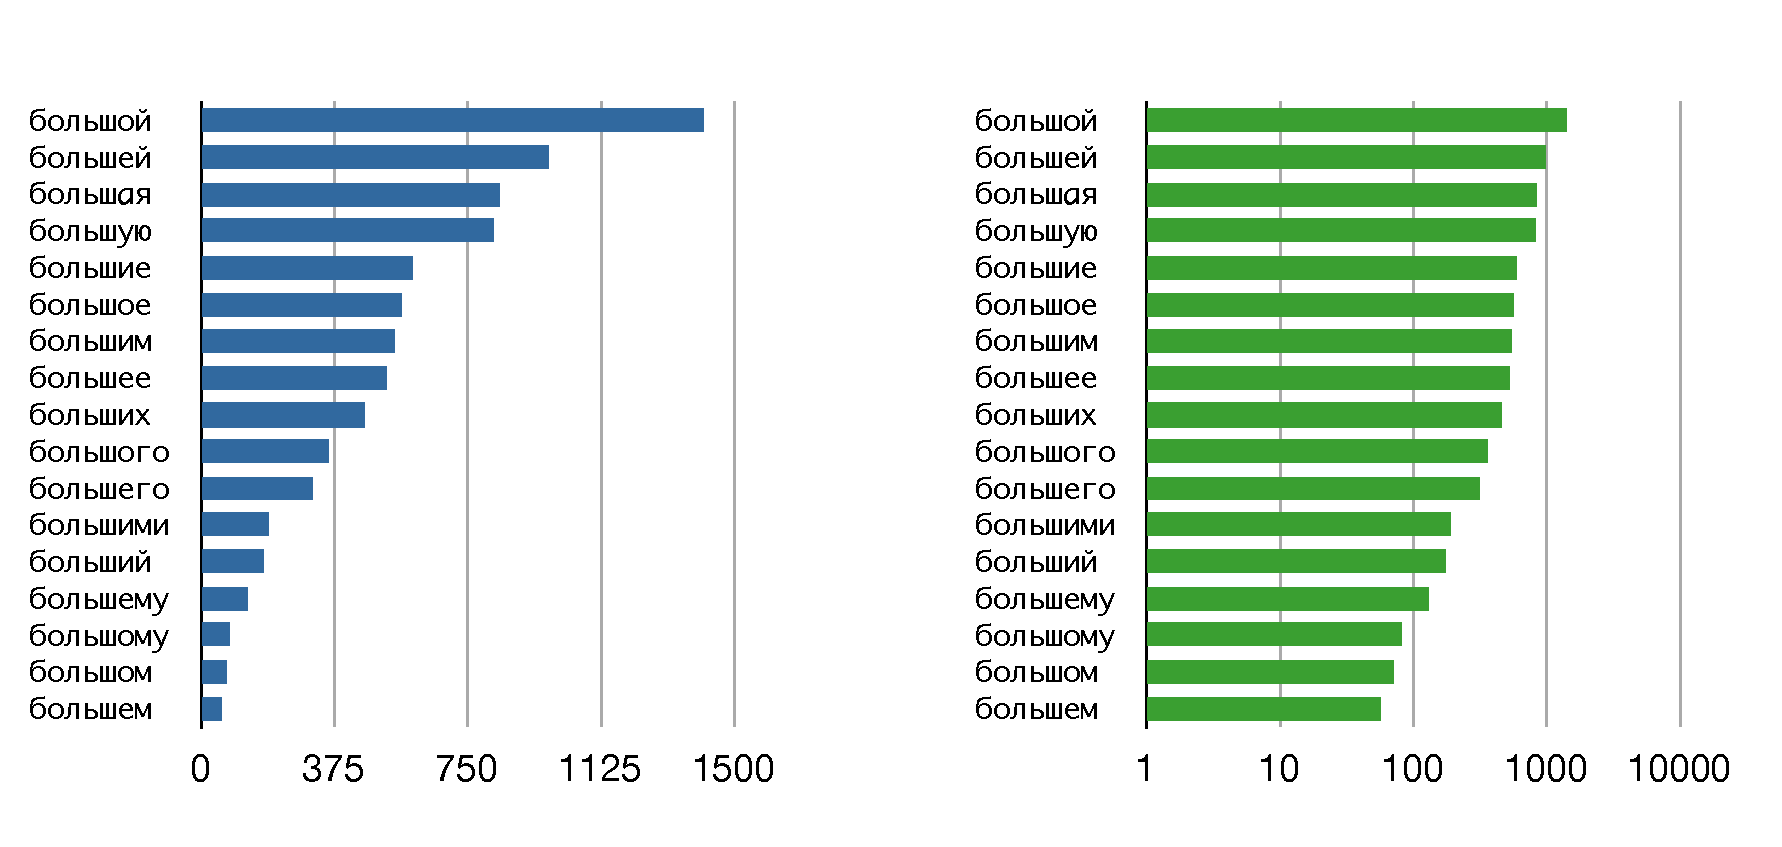
\includegraphics[width=0.75\textwidth]{fig/frequencies}
  \caption{Frequencies and log frequencies of various inflections of a Russian adjective (meaning \textit{large}) taken from our corpus}
  \label{fig:freq}
\end{figure}

\subsection{Implementation}
Inference is done for this model using collapsed Gibbs sampling, whith the Chinese restaurant process (CRP) representation and two collapsed Dirichlet-multinomials for the base distribution.

Our implementation alternatively considers assignments of tokens to tables in the CRP and segmentations of words in the base distributions into a prefix, suffix pair. These two types of latent variables are resampled iteratively until convergence indicated by the marginal likelihood of the model.

Finally, we proceed to decode each word in the corpus into its prefix, suffix pair by finding the most likely segmentation for each type according to the base distribution: $\max_{s,p} p(p \mid \theta_p) p(s \mid \theta_s)$.

\subsection{Limitations}

While the implementation of the baseline model using Gibbs sampling has the advantage of being straightforward and easily extendable to incorporate more complex morphology, it suffers from being very inefficient. This is due to the process of sampling table assignments in the CRP representation, which requires keeping track of data structures that are constantly updated. Although some effort has been made \cite{blunsom2009} to make these structures more efficient, these improvements would have very little effect in our case because of the low number of tables involved.

One practical solution would be to abandon the frequencies completely and directly model the types, but one would loose all the potential contextual information present at the token level. In the following, we propose a more generic approach which attempts to overcome the time requirements of learning with CRP sampling by introducing independencies in the model which allow parallelization of the inference procedure.

